

\subsubsection{History of computers vs Humans}
In 1997, Deep Blue a computer built by IBM won a six games match against the current chess world champion Garry Kasparov. Humans got beaten on Chess, but remain undefeated on Go, therefore the research has switched to that game. Until 2002, methods based on decompositions and positions evaluations were used in order to solve such games. From 2002 to 2005 the Monte Carlo algorithm was used in order to find the best moves. Since 2006, it's implementation in a tree (MCTS) has been developped, rocketing the results in term of Artificial Intelligence on Go. On june 5th, 2013, Zen a Go programm defeated Takuto Ooomote (9 Dan) with a 3 stone handicap.\cite{computer_Go_vs_human}
\begin{figure}[H]
\centering
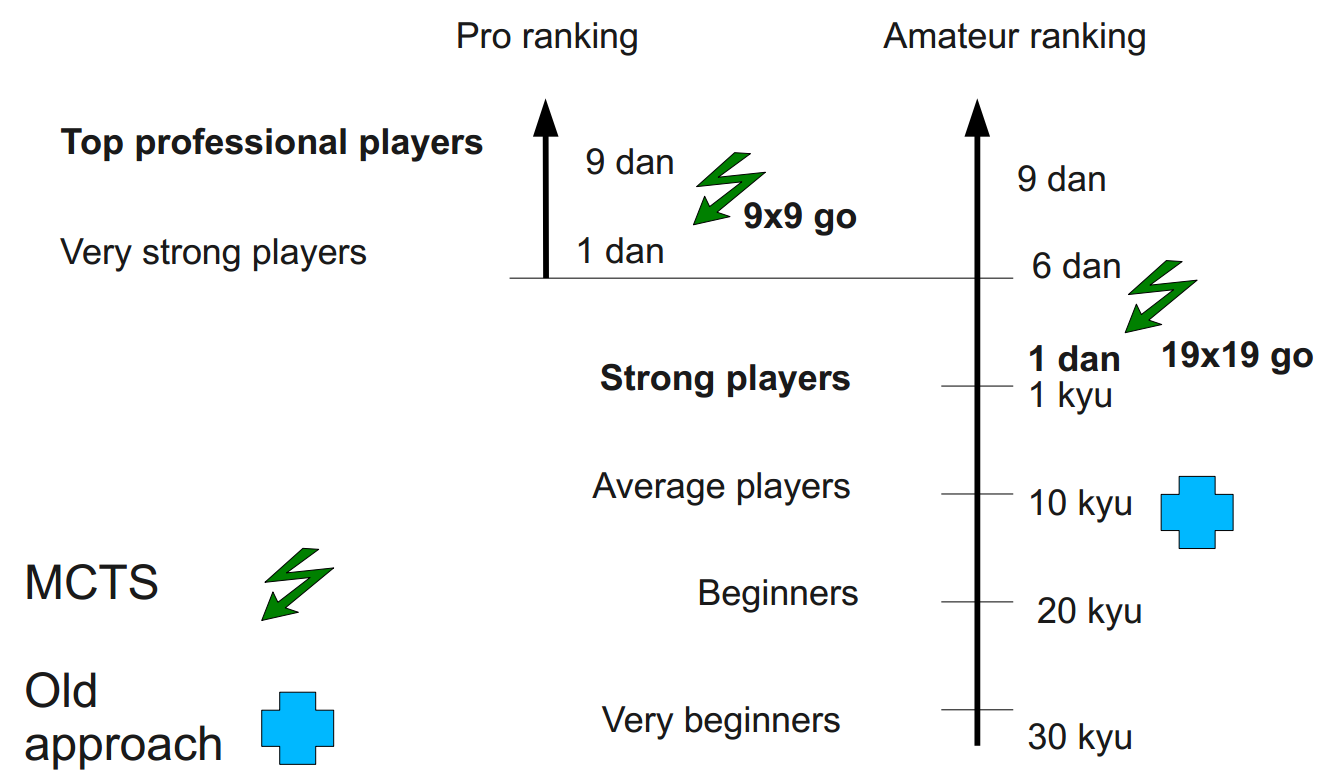
\includegraphics[width=12cm]{2_State_of_the_art/Arimaa_on_MCTS_Benoit/img/ranking.png}
\caption{\label{fig:ranking}Comparison between Go algorithms and human skill (\textit{2011}).}
\end{figure}
\textit{The ranking system of the game of Go is the following : kyu are for students ranks, Dan are masters ranks. Beginners start at 30 kyu and advance downward the kyu grades. Once one ranks over 1 kyu, he will receive the 1st Dan (as the black belt in Judo) and will move upward through the Dan ranks until the 9th.}\\
However MCTS wasn't the first method applied in order to solve Arimaa, the \ensuremath{\alpha\beta} method was used first. At the moment the top programms (Bomb by David Fotland : 2002 to 2008, Clueless by Jeff Bacher 2009) are ranked about 1800 elo\footnote{\textit{The Elo rating system is a method for calculating the relative skill levels of players in competitor-versus-competitor games such as chess. It use also used for Arimaa. Beginers rank around 1200 elo, experts around 2000 elo and International Masters over 2400 elo.}}. For comparison, strongest humans players are rated around 2450 elo.\cite{master_mcts_kozeleck}
\medskip
